%%%%%%%%%%%%%%%%%%%%%%%%%%%%%%%%%%%%%%%%%
% Jacobs Landscape Poster
% LaTeX Template
% Version 1.1 (14/06/14)
%
% Created by:
% Computational Physics and Biophysics Group, Jacobs University
% https://teamwork.jacobs-university.de:8443/confluence/display/CoPandBiG/LaTeX+Poster
% 
% Further modified by:
% Nathaniel Johnston (nathaniel@njohnston.ca)
%
% This template has been downloaded from:
% http://www.LaTeXTemplates.com
%
% License:
% CC BY-NC-SA 3.0 (http://creativecommons.org/licenses/by-nc-sa/3.0/)
%
%%%%%%%%%%%%%%%%%%%%%%%%%%%%%%%%%%%%%%%%%

%----------------------------------------------------------------------------------------
%	PACKAGES AND OTHER DOCUMENT CONFIGURATIONS
%----------------------------------------------------------------------------------------

\documentclass[final]{beamer}

\usepackage[scale=1.24]{beamerposter}

\usetheme{confposter}

\setbeamercolor{block title}{fg=dblue,bg=white}
\setbeamercolor{block body}{fg=black,bg=white}
\setbeamercolor{block alerted title}{fg=white,bg=dblue!70}
\setbeamercolor{block alerted body}{fg=black,bg=dblue!10}
\setbeamercolor{item}{fg=nblue}
\setbeamercolor{item projected}{fg=white,bg=nblue}

\newcommand{\emphone}[1]{\textit{\color{norange}#1}}



%-----------------------------------------------------------
% Define the column widths and overall poster size
% To set effective sepwid, onecolwid and twocolwid values, first choose how many columns you want and how much separation you want between columns
% In this template, the separation width chosen is 0.024 of the paper width and a 4-column layout
% onecolwid should therefore be (1-(# of columns+1)*sepwid)/# of columns e.g. (1-(4+1)*0.024)/4 = 0.22
% Set twocolwid to be (2*onecolwid)+sepwid = 0.464
% Set threecolwid to be (3*onecolwid)+2*sepwid = 0.708

\newlength{\sepwid}
\newlength{\onecolwid}
\newlength{\twocolwid}
\newlength{\threecolwid}
\setlength{\paperwidth}{46.8in} % A0 width: 46.8in
\setlength{\paperheight}{33.1in} % A0 height: 33.1in
\setlength{\sepwid}{0.024\paperwidth} % Separation width (white space) between columns
\setlength{\onecolwid}{0.22\paperwidth} % Width of one column
\setlength{\twocolwid}{0.464\paperwidth} % Width of two columns
\setlength{\threecolwid}{0.708\paperwidth} % Width of three columns
\setlength{\topmargin}{-1.5in} % Reduce the top margin size
%-----------------------------------------------------------

\usepackage{kmath}
% ------------------------ %
% 	  Packages		%
% ------------------------ %

\usepackage[utf8]{inputenc}
\usepackage[T1]{fontenc}
\usepackage{xparse}
\usepackage{pgffor}
\usepackage{ifthen}
\usepackage{xspace}
\usepackage{xcolor}
\usepackage{amsmath}
\usepackage{amssymb}
\usepackage{amsfonts}
\usepackage{amsthm}
\usepackage{mathrsfs}
\usepackage{bbm}
\usepackage{mathtools}
\usepackage{stmaryrd}
\usepackage[ruled,linesnumbered]{algorithm2e}
\newcommand\mycommfont[1]{\footnotesize\ttfamily\textcolor{blue}{#1}}
\SetCommentSty{mycommfont}
\usepackage{csquotes}
\usepackage{dblfloatfix}
\usepackage{comment}
\renewcommand{\ttdefault}{lmtt}


% ------------------------ %
% 	  Shortcuts		  %
% ------------------------ %


% Lowercase styles
\foreach \x in {a,...,z}{%
	\expandafter\xdef\csname \x\endcsname{\noexpand\ensuremath{\noexpand\mathbf{\x}}}
}
\foreach \x in {a,...,z}{%
	\expandafter\xdef\csname \x rm\endcsname{\noexpand\ensuremath{\noexpand\mathrm{\x}}}
}

% Uppercase styles
\foreach \x in {A,...,Z}{%
	\expandafter\xdef\csname \x\endcsname{\noexpand\ensuremath{\noexpand\mathbf{\x}}}
}
\foreach \x in {A,...,Z}{%
	\expandafter\xdef\csname \x rm\endcsname{\noexpand\ensuremath{\noexpand\mathrm{\x}}}
}
\foreach \x in {A,...,Z}{%
	\expandafter\xdef\csname \x bb\endcsname{\noexpand\ensuremath{\noexpand\mathbb{\x}}}
}
\foreach \x in {A,...,Z}{%
	\expandafter\xdef\csname \x c\endcsname{\noexpand\ensuremath{\noexpand\mathcal{\x}}}
}

% Figures styles
\def\0{{\mathbf 0}}
\def\1{{\mathbf 1}}

% Miscellaneous
\def\ie{\textit{i.e.}}
\def\eg{\textit{e.g.}}
\def\etal{\textit{et al.}}
\def\resp{\textit{resp.}}

% Notes
\def\addNote#1{{\noindent\color{blue}{[Note : #1]}}}
\def\toDo#1{{\noindent\color{red}{[Todo : #1]}}}
\def\addCite{{\noindent\color{orange}{[Cite] }}}


% ------------------------------  %
% 			Macros 		   	  %
% ------------------------------  %

% Problems
\newcommand{\primal}{\mathcal{P}\xspace}
\newcommand{\dual}{\mathcal{D}\xspace}
\newcommand{\opt}[1]{\ensuremath{{{#1}^{\star}}}\xspace}

% Regularizer
\newcommand{\rego}{\ensuremath{\lambda}\xspace}
\newcommand{\regt}{\ensuremath{\gamma}\xspace}

% Primal
\newcommand{\pfunc}{\ensuremath{P}\xspace}
\newcommand{\pve}{\ensuremath{x}\xspace}
\newcommand{\pv}{\ensuremath{\mathbf{\pve}}\xspace}
\newcommand{\pveopt}{\ensuremath{\pve^\star}\xspace}
\newcommand{\pvopt}{\ensuremath{\pv^\star}\xspace}
\newcommand{\pvew}{\ensuremath{\tilde{\pve}}\xspace}
\newcommand{\pvw}{\ensuremath{\tilde{\pv}}\xspace}
\newcommand{\pvewopt}{\ensuremath{\pvew^\star}\xspace}
\newcommand{\pvwopt}{\ensuremath{\pvw^\star}\xspace}
\newcommand{\pr}{\ensuremath{{\mathcal{X}}}\xspace}

% Dual
\newcommand{\dfunc}{\ensuremath{D}\xspace}
\newcommand{\dve}{\ensuremath{u}\xspace}
\newcommand{\dv}{\ensuremath{\mathbf{\dve}}\xspace}
\newcommand{\dveopt}{\ensuremath{\dve^\star}\xspace}
\newcommand{\dvopt}{\ensuremath{\dv^\star}\xspace}
\newcommand{\dvew}{\ensuremath{\tilde{\dve}}\xspace}
\newcommand{\dvw}{\ensuremath{\tilde{\dv}}\xspace}
\newcommand{\dvewopt}{\ensuremath{\dvew^\star}\xspace}
\newcommand{\dvwopt}{\ensuremath{\dvw^\star}\xspace}
\newcommand{\dr}{\ensuremath{{\mathcal{U}}}\xspace}

% Variable
\newcommand{\obs}{\ensuremath{\y}\xspace}
\newcommand{\dicintro}{\ensuremath{\D}\xspace}
\newcommand{\dic}{\ensuremath{\A}\xspace}
\newcommand{\atom}{\ensuremath{\a}\xspace}
\newcommand{\Id}{\ensuremath{\I}\xspace}
\newcommand{\values}{\ensuremath{\boldsymbol{\eta}}\xspace}

% Dimensions
\newcommand{\pdim}{\ensuremath{n}\xspace}
\newcommand{\ddim}{\ensuremath{m}\xspace}

% Regions
\newcommand{\region}{\ensuremath{{\mathcal{R}}}\xspace}
\newcommand{\sphere}{\ensuremath{{\mathcal{S}}}\xspace}

% Sets
\newcommand{\set}{\ensuremath{\mathcal{I}}\xspace}
\newcommand{\cset}{\ensuremath{\bar{\set}}\xspace}
\newcommand{\nset}{\ensuremath{\set_{\bullet}}\xspace}
\newcommand{\setnull}{\ensuremath{{\mathcal{\set}_0}}\xspace}
\newcommand{\setnullopt}{\ensuremath{{\mathcal{\set}_0^\star}}\xspace}
\newcommand{\setnulloptcomp}{\ensuremath{{\overline{\mathcal{\set}}_0^\star}}\xspace}
\newcommand{\setpos}{\ensuremath{{\mathcal{\set}_+}}\xspace}
\newcommand{\setposcmp}{\ensuremath{{\overline{\mathcal{\set}}_+}}\xspace}
% \newcommand{\setposopt}{\ensuremath{\mathcal{\set}_+^\star}\xspace}
\newcommand{\setposopt}{\ensuremath{\mathcal{J}^\star}\xspace}
\newcommand{\setposoptcmp}{\ensuremath{\overline{\mathcal{\set}}_+^\star}\xspace}
\newcommand{\setscreen}{\ensuremath{{\mathcal{I}}}\xspace}
\newcommand{\setscreenc}{\ensuremath{{\overline{\mathcal{I}}}}\xspace}
\newcommand{\setrelax}{\ensuremath{{\mathcal{J}}}\xspace}
\newcommand{\setrelaxc}{\ensuremath{{\overline{\mathcal{J}}}}\xspace}
\newcommand{\setsr}{\ensuremath{{\mathcal{K}}}\xspace}
\newcommand{\setsrc}{\ensuremath{{\overline{\mathcal{K}}}}\xspace}
\newcommand{\setopt}{\ensuremath{{\mathcal{\set}}^\star}\xspace}
% \newcommand{\setscreen}{\ensuremath{{\mathcal{\set}_s}}\xspace}
% \newcommand{\setscreenc}{\ensuremath{{\overline{\mathcal{\set}}_s}}\xspace}
% \newcommand{\setrelax}{\ensuremath{{\mathcal{\set}_r}}\xspace}
% \newcommand{\setrelaxc}{\ensuremath{{\overline{\mathcal{\set}}_r}}\xspace}

% Operators
\newcommand{\argmin}[1]{\ensuremath{\underset{#1}{\mathrm{argmin}}}\xspace}
\newcommand{\argmax}[1]{\ensuremath{\underset{#1}{\mathrm{argmax}}}\xspace}
\newcommand{\scalprod}[2]{\ensuremath{\langle{#1,#2}\rangle}\xspace}
\newcommand{\card}[1]{\ensuremath{\mathrm{card}(#1)}\xspace}
\newcommand{\conj}[1]{\ensuremath{#1^{\star}}\xspace}
\newcommand{\proj}[2]{\ensuremath{\mathrm{proj}_{#2}(#1)}\xspace}
\newcommand{\prox}[2]{\ensuremath{\mathrm{prox}_{#2}(#1)}\xspace}
\newcommand{\gap}[2]{\ensuremath{\mathrm{gap}({#1},{#2})}\xspace}
\newcommand{\supp}[1]{\ensuremath{\mathrm{supp}({#1})}\xspace}
\newcommand{\abs}[1]{\ensuremath{|#1|}\xspace}
\newcommand{\norm}[1]{\ensuremath{\|#1\|}\xspace}
\newcommand{\normZ}[1]{\ensuremath{\|#1\|_0}\xspace}
\newcommand{\normO}[1]{\ensuremath{\|#1\|_1}\xspace}
\newcommand{\normT}[1]{\ensuremath{\|#1\|_2}\xspace}
\newcommand{\transp}[1]{\ensuremath{#1^{T}}\xspace}
\newcommand{\sign}[1]{\ensuremath{\mathrm{sign}({#1})}\xspace}
\newcommand{\diff}[2]{\ensuremath{\frac{\partial#1}{\partial#2}}\xspace}
\DeclarePairedDelimiter\ceil{\lceil}{\rceil}
\DeclarePairedDelimiter\floor{\lfloor}{\rfloor}

\newcommand{\intervint}[2]{\llbracket#1,#2\rrbracket}
\newcommand{\idxpvel}{i}
\newcommand{\idxscreen}{\ell}
\newcommand{\idxrelax}{\ell}
\newcommand{\subgrad}{\mathbf{g}}
\newcommand{\setnz}{\mathcal{I}^\star}

\newcommand{\ones}{{\bf1}}

\newcommand{\safesphere}{\mathcal{S}}
\newcommand{\spherec}{\dv}
\newcommand{\spherer}{r}

% Closed-form expression quantities
\newcommand{\matxpos}{\B}
\newcommand{\matcorrpos}{\G}
\newcommand{\vecxpos}{\b}

% sub-problem quantities
\newcommand{\reducedNormOne}{\mathbf{v}}
\newcommand{\reducedNormTwo}{\M}
\newcommand{\obsred}{\obs_r}
\newcommand{\pvred}{\pv_r}
\newcommand{\dicred}{\dic_r}
\newcommand{\pdimred}{\pdim_r}
\newcommand{\pfunred}{\pfun_r}


% Rank-one update data
\newcommand{\permat}{\P}
\newcommand{\dicobs}{\v}
\newcommand{\dicobsrego}{\w}
\newcommand{\dicobsregoe}{w}
\newcommand{\gramposi}{\g_1}
\newcommand{\gramnulli}{\g_2}
\newcommand{\gramii}{q}
\newcommand{\graminvgramposi}{\r}
\newcommand{\outerprod}{\R}
\newcommand{\lowerightblock}{d}
\newcommand{\matxposred}{\tilde{\matxpos}}

% Proofs
\newcommand{\multipl}{\boldsymbol{\mu}}
\newcommand{\sphereray}{\boldsymbol{\tau}}
\usepackage{graphicx}
\usepackage{booktabs}
\usepackage{parskip}

\usepackage[pscoord]{eso-pic}
\newcommand{\placetextbox}[3]{
  \setbox0=\hbox{#3}
  \AddToShipoutPictureFG*{
    \put(\LenToUnit{#1\paperwidth},\LenToUnit{#2\paperheight}){\vtop{{\null}\makebox[0pt][c]{#3}}}
  }
}

%----------------------------------------------------------------------------------------
%	TITLE SECTION 
%----------------------------------------------------------------------------------------

\title{Screen \& Relax : Accelerating the resolution of the Elastic-Net} % Poster title

\author{Théo Guyard${}^{\star}$, Cédric Herzet${}^{\dagger}$, Clément Elvira${}^{\ddagger}$} % Author(s)

\institute{${}^{\star}$Applied Mathematics Department, INSA Rennes, France | ${}^{\dagger}$SIMSMART team, INRIA Rennes-Bretagne Atlantique, France | ${}^{\ddagger}$SCEE team, CentraleSupelec Rennes, France} % Institution(s)

%----------------------------------------------------------------------------------------

\begin{document}

\placetextbox{0.955}{0.995}{\fbox{Paper ID : 2487}}

\addtobeamertemplate{block end}{}{\vspace*{2ex}} % White space under blocks
\addtobeamertemplate{block alerted end}{}{\vspace*{2ex}} % White space under highlighted (alert) blocks

\setlength{\belowcaptionskip}{2ex} % White space under figures
\setlength\belowdisplayshortskip{2ex} % White space under equations

\begin{frame}[t] % The whole poster is enclosed in one beamer frame

\begin{columns}[t]

\begin{column}{\sepwid}\end{column}

\begin{column}{\onecolwid}
    \begin{alertblock}{Objectives}
        Accelerate the resolution of the Elastic-Net :
        \begin{itemize}
            \item \hspace{0.1in} Identification of \emphone{zeros} in the optimizer
            \item \hspace{0.1in} Identification of \emphone{non-zeros} in the optimizer
            \item \hspace{0.1in} Reduction of the problem dimension
            \item \hspace{0.1in} Reduction of the complexity burden
        \end{itemize}
    \end{alertblock}
    \begin{block}{Problem of interest}
        \begin{itemize}
            \item \hspace{0.1in} Sparse decomposition aims at finding some approximation of a vector \(\obs\) as the linear combination of a few columns of a dictionary \(\dic\).
            The Elastic-Net is one way to achieve this :
        \end{itemize}
        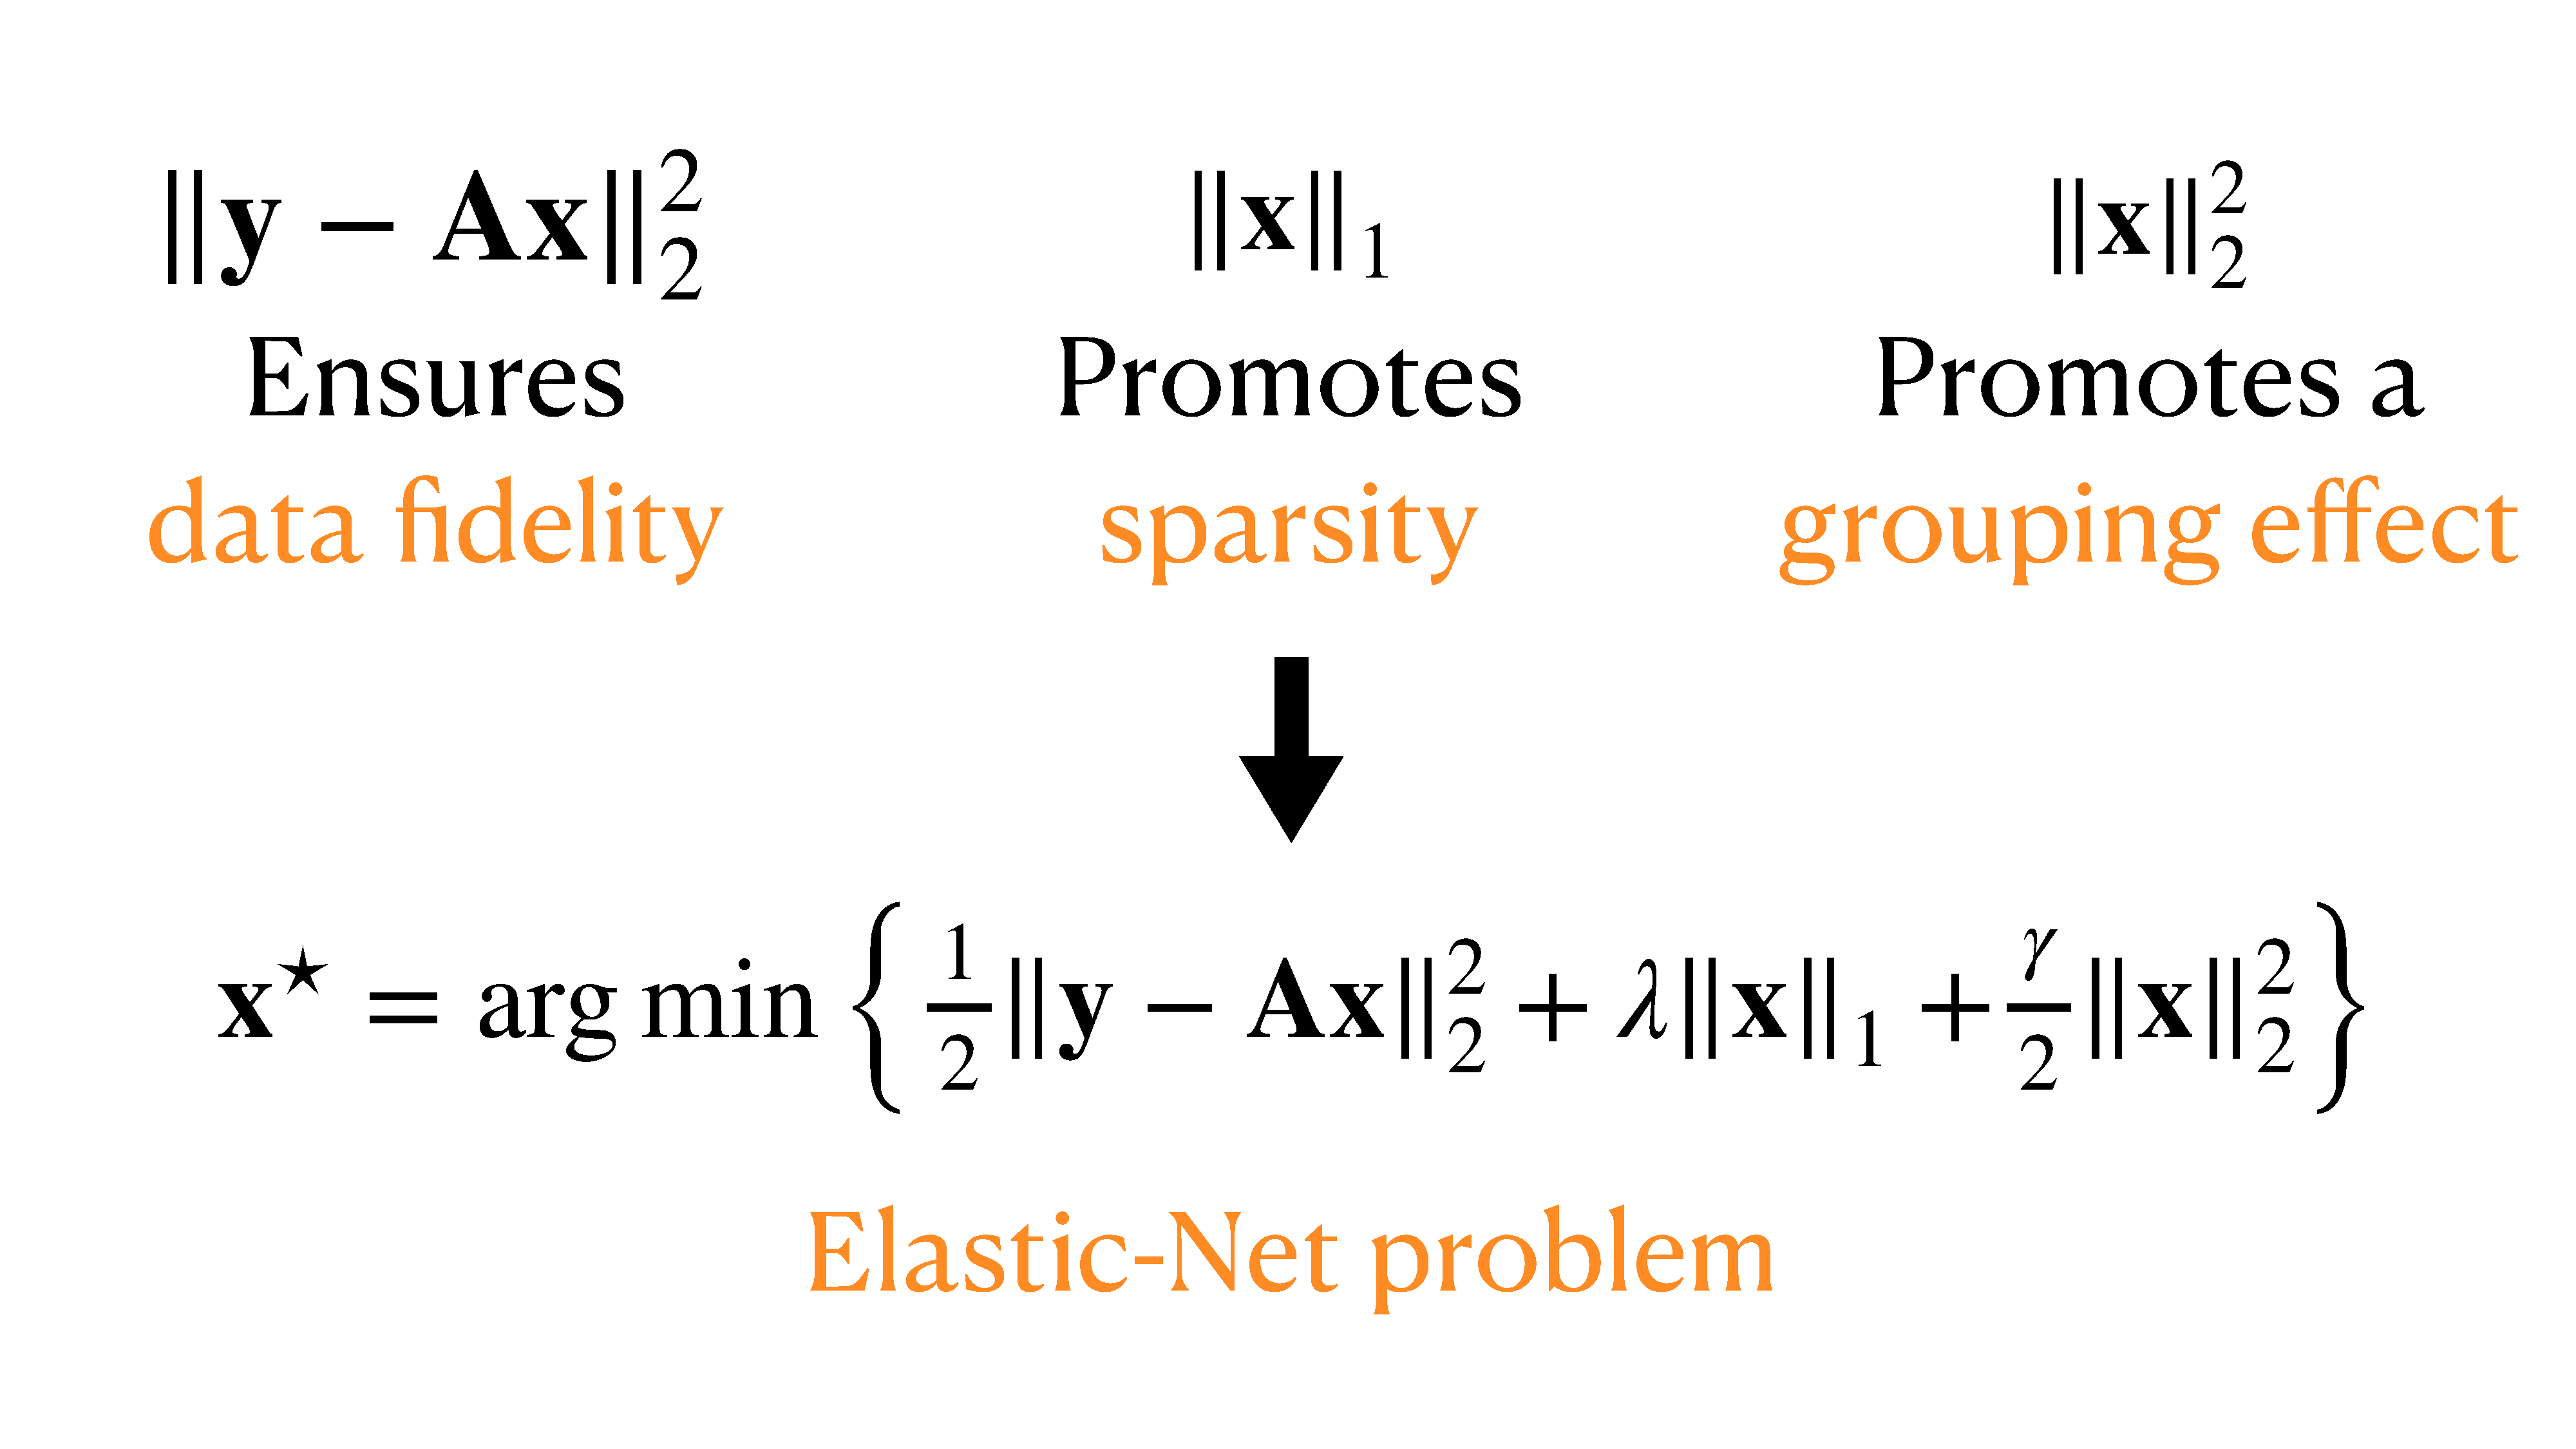
\includegraphics[width=\linewidth]{elastic-net.pdf}
        \vspace{-2cm}
        \begin{itemize}
            \item \hspace{0.1in} The Elastic-Net is a convex problem so gradient-based methods are particularity well suited to solve it :
        \end{itemize}
        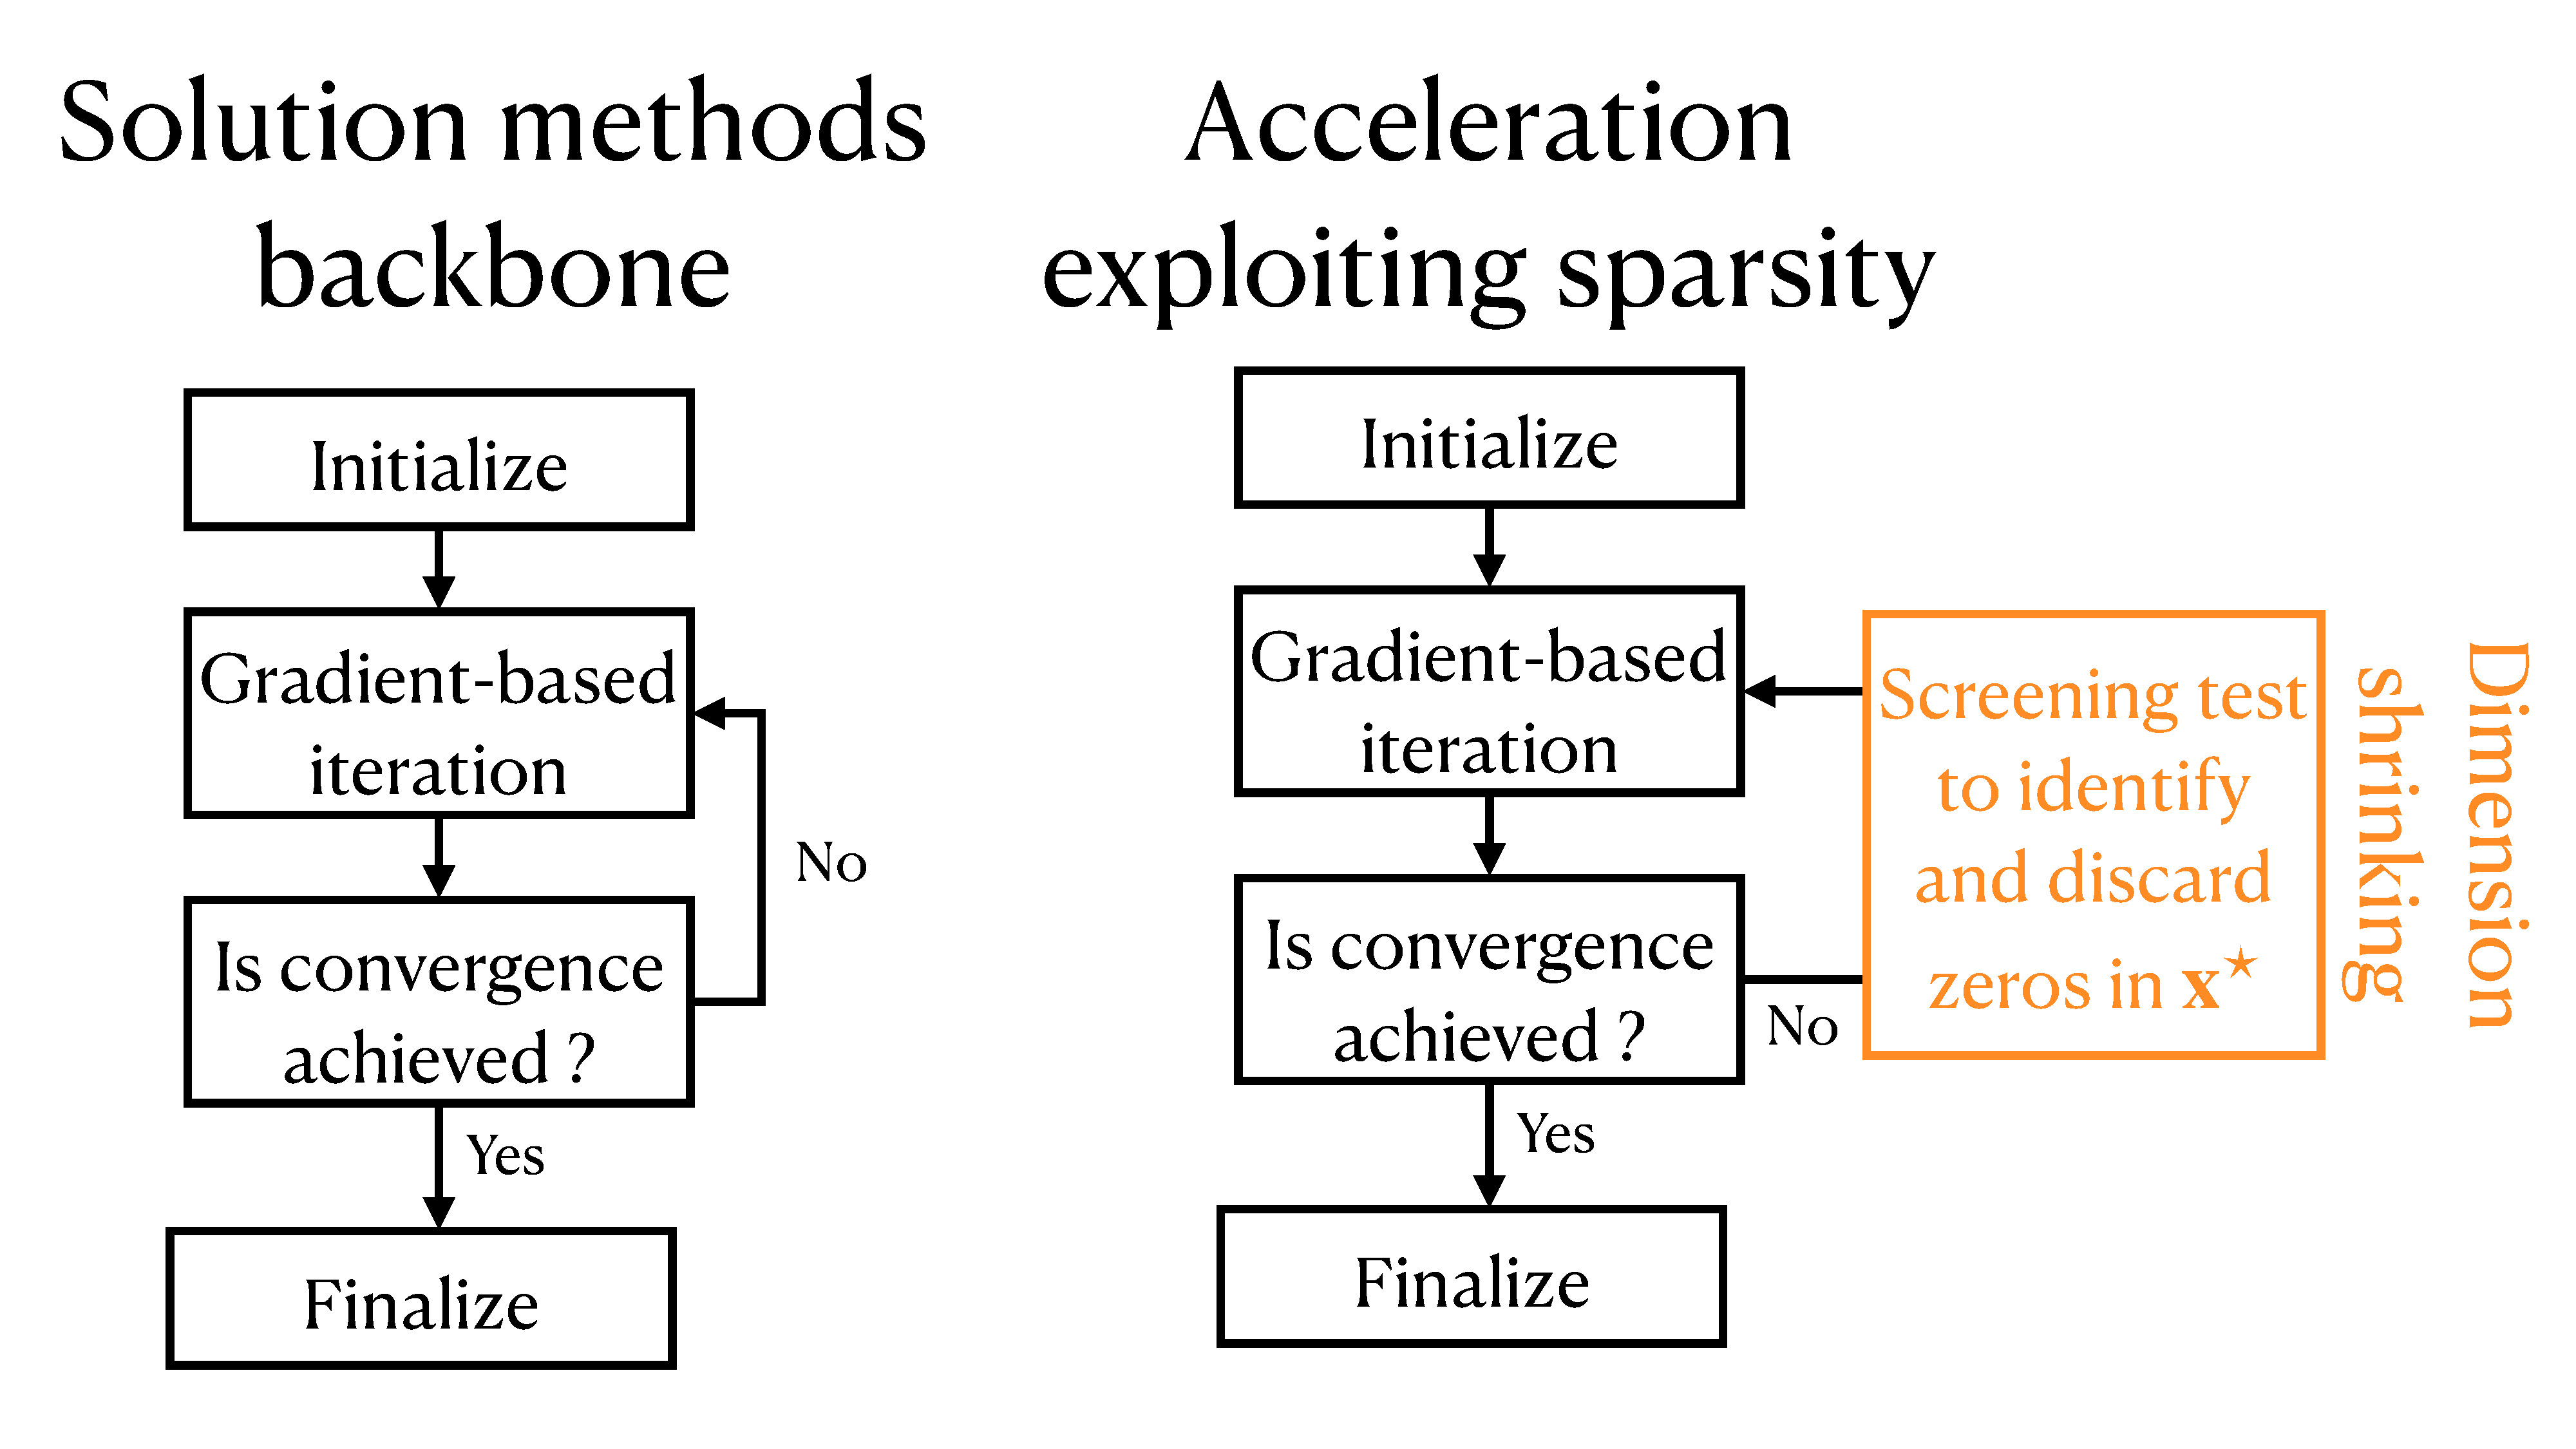
\includegraphics[width=\linewidth]{solution-method.pdf}
        \vspace{-1cm}
        \begin{itemize}
            \item \hspace{0.1in} Our initial idea :
            \begin{itemize}
                \normalsize \item[-] \hspace{0.1in} \normalsize Why not identifying \emphone{non-zeros} in $\pvopt$ ?
                \item[-] \hspace{0.1in} \normalsize We could break the non-differentiability of the $\ell_1$-norm at zero ...
                \item[-] \hspace{0.1in} \normalsize This potentially allows to shrink even more the problem dimension !
            \end{itemize}
        \end{itemize}
    \end{block}
\end{column}

\begin{column}{\sepwid}\end{column}

\begin{column}{\twocolwid}
    \begin{block}{Let's play with duality !}
        \begin{columns}[t,totalwidth=\twocolwid]
            \begin{column}{\onecolwid}
                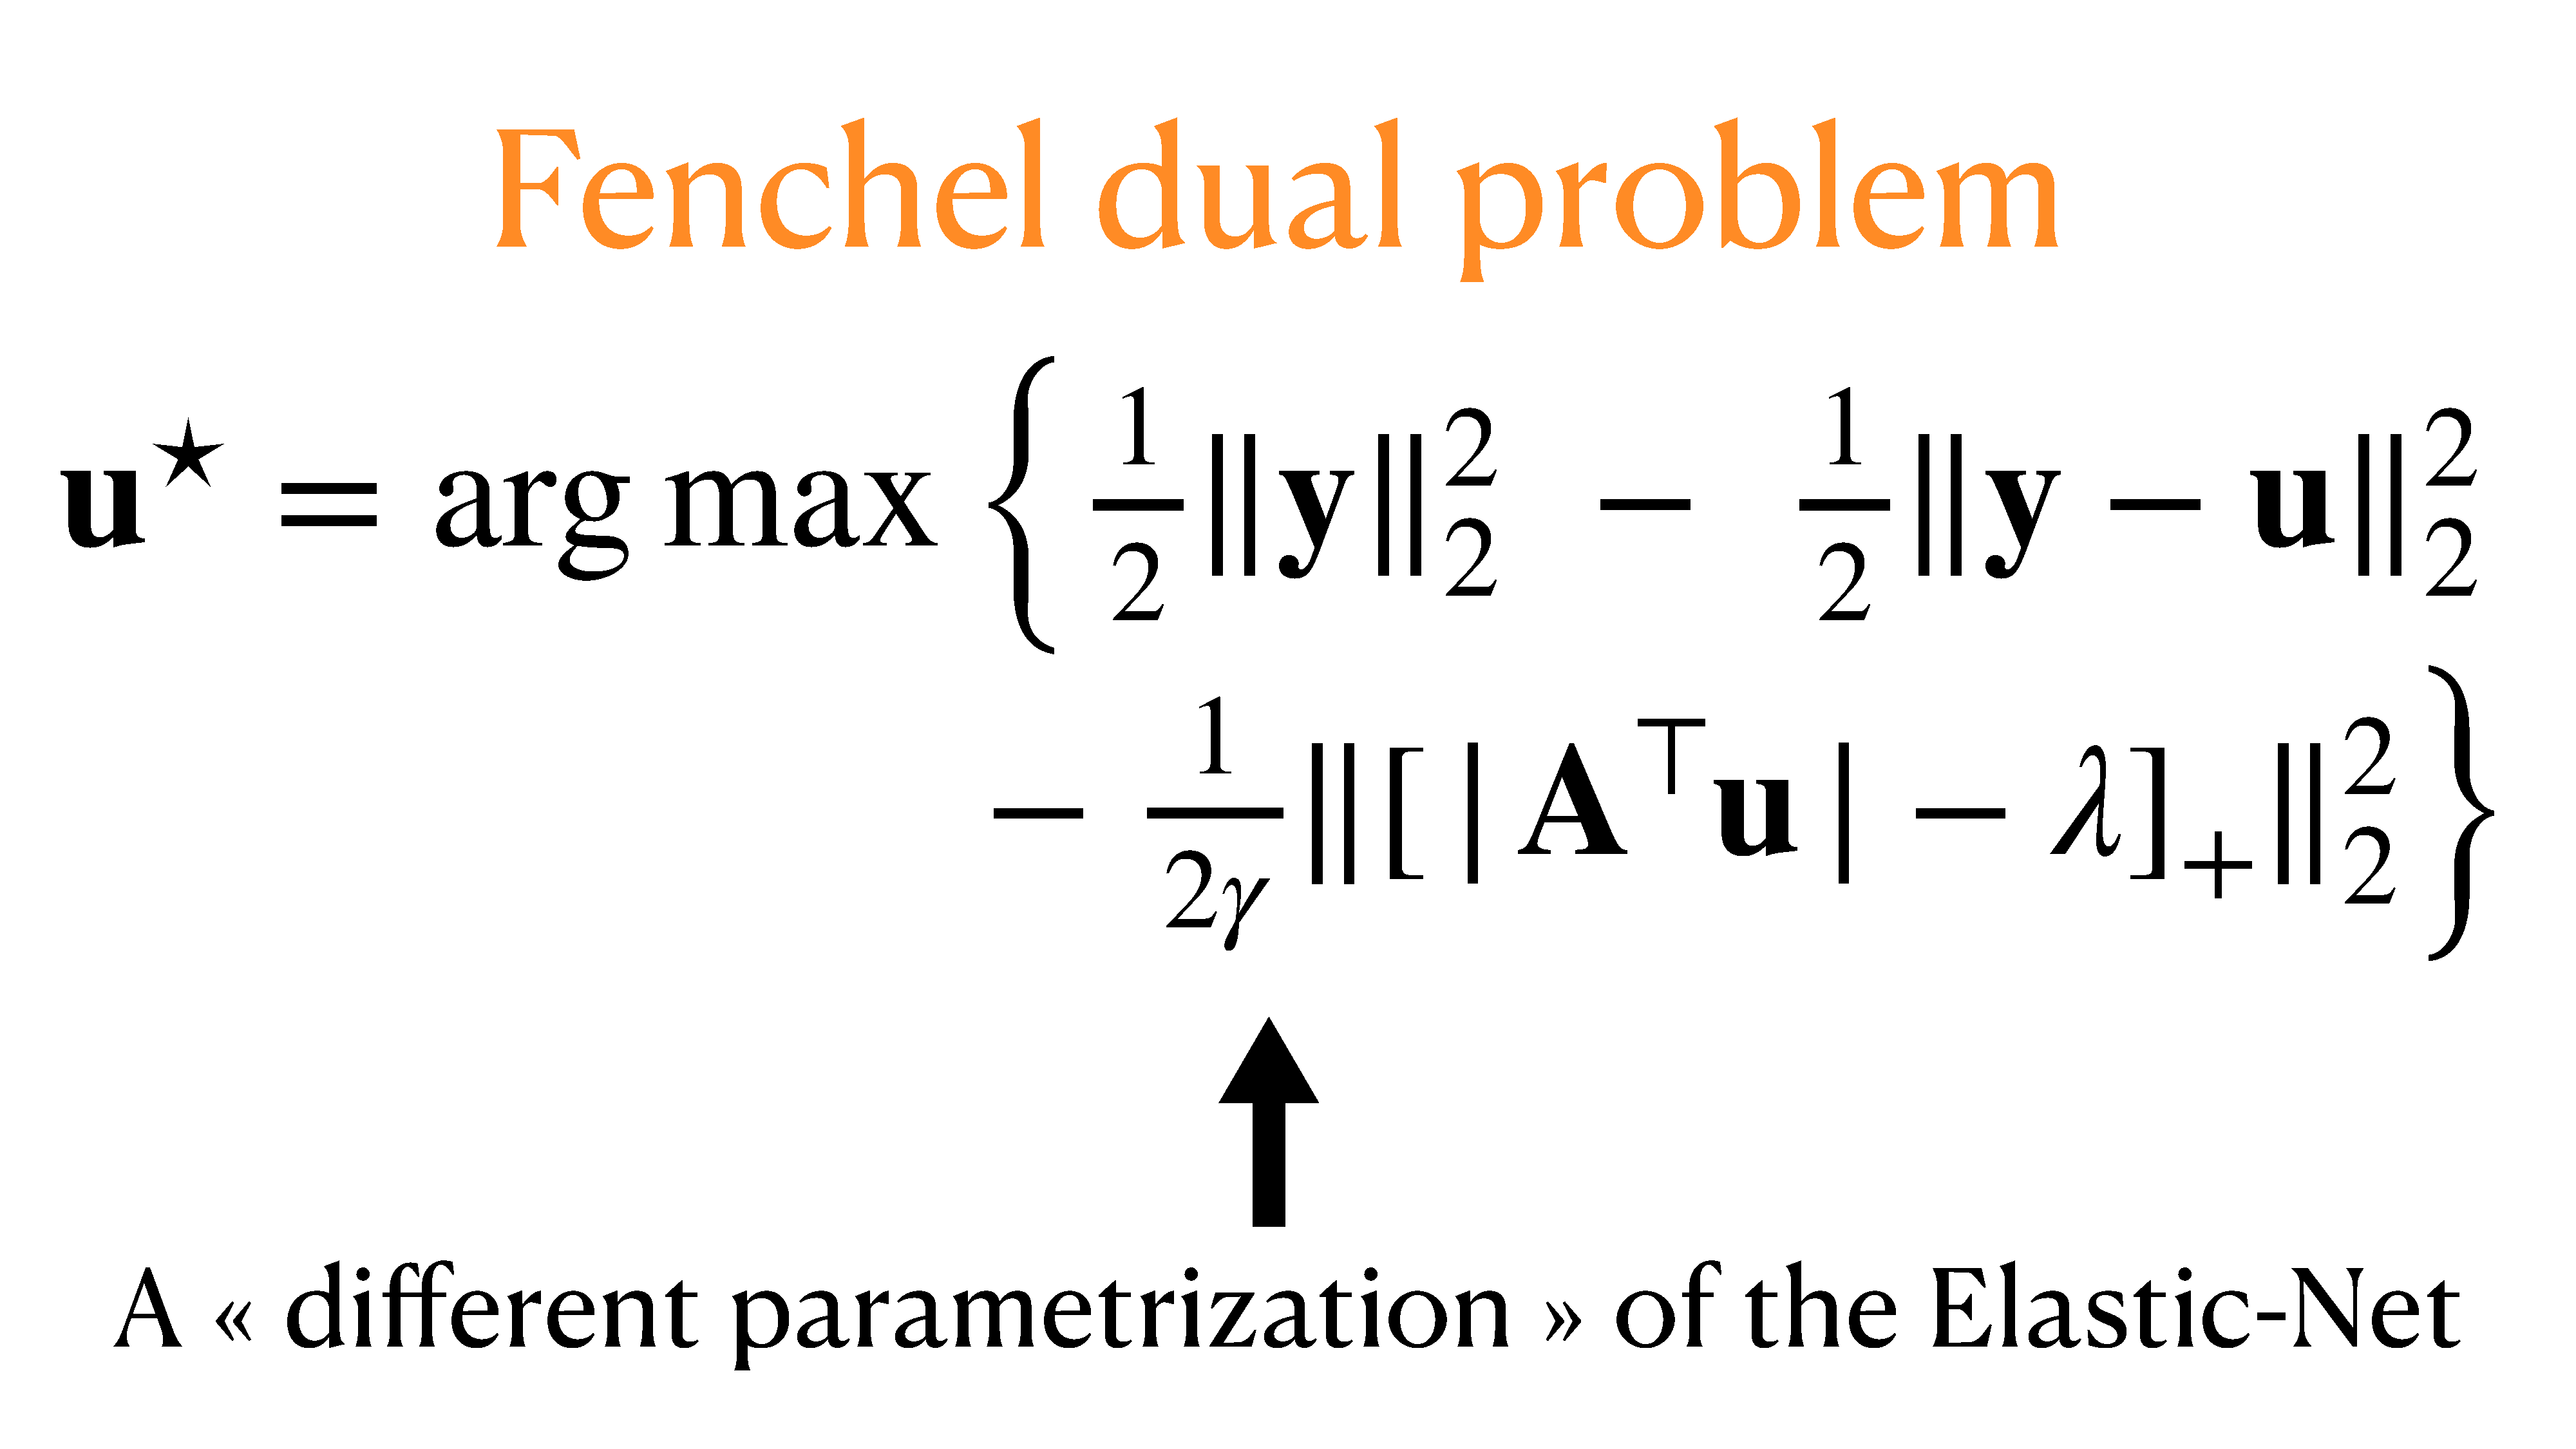
\includegraphics[width=\linewidth]{dual.pdf}
            \end{column}
            \begin{column}{\onecolwid}
                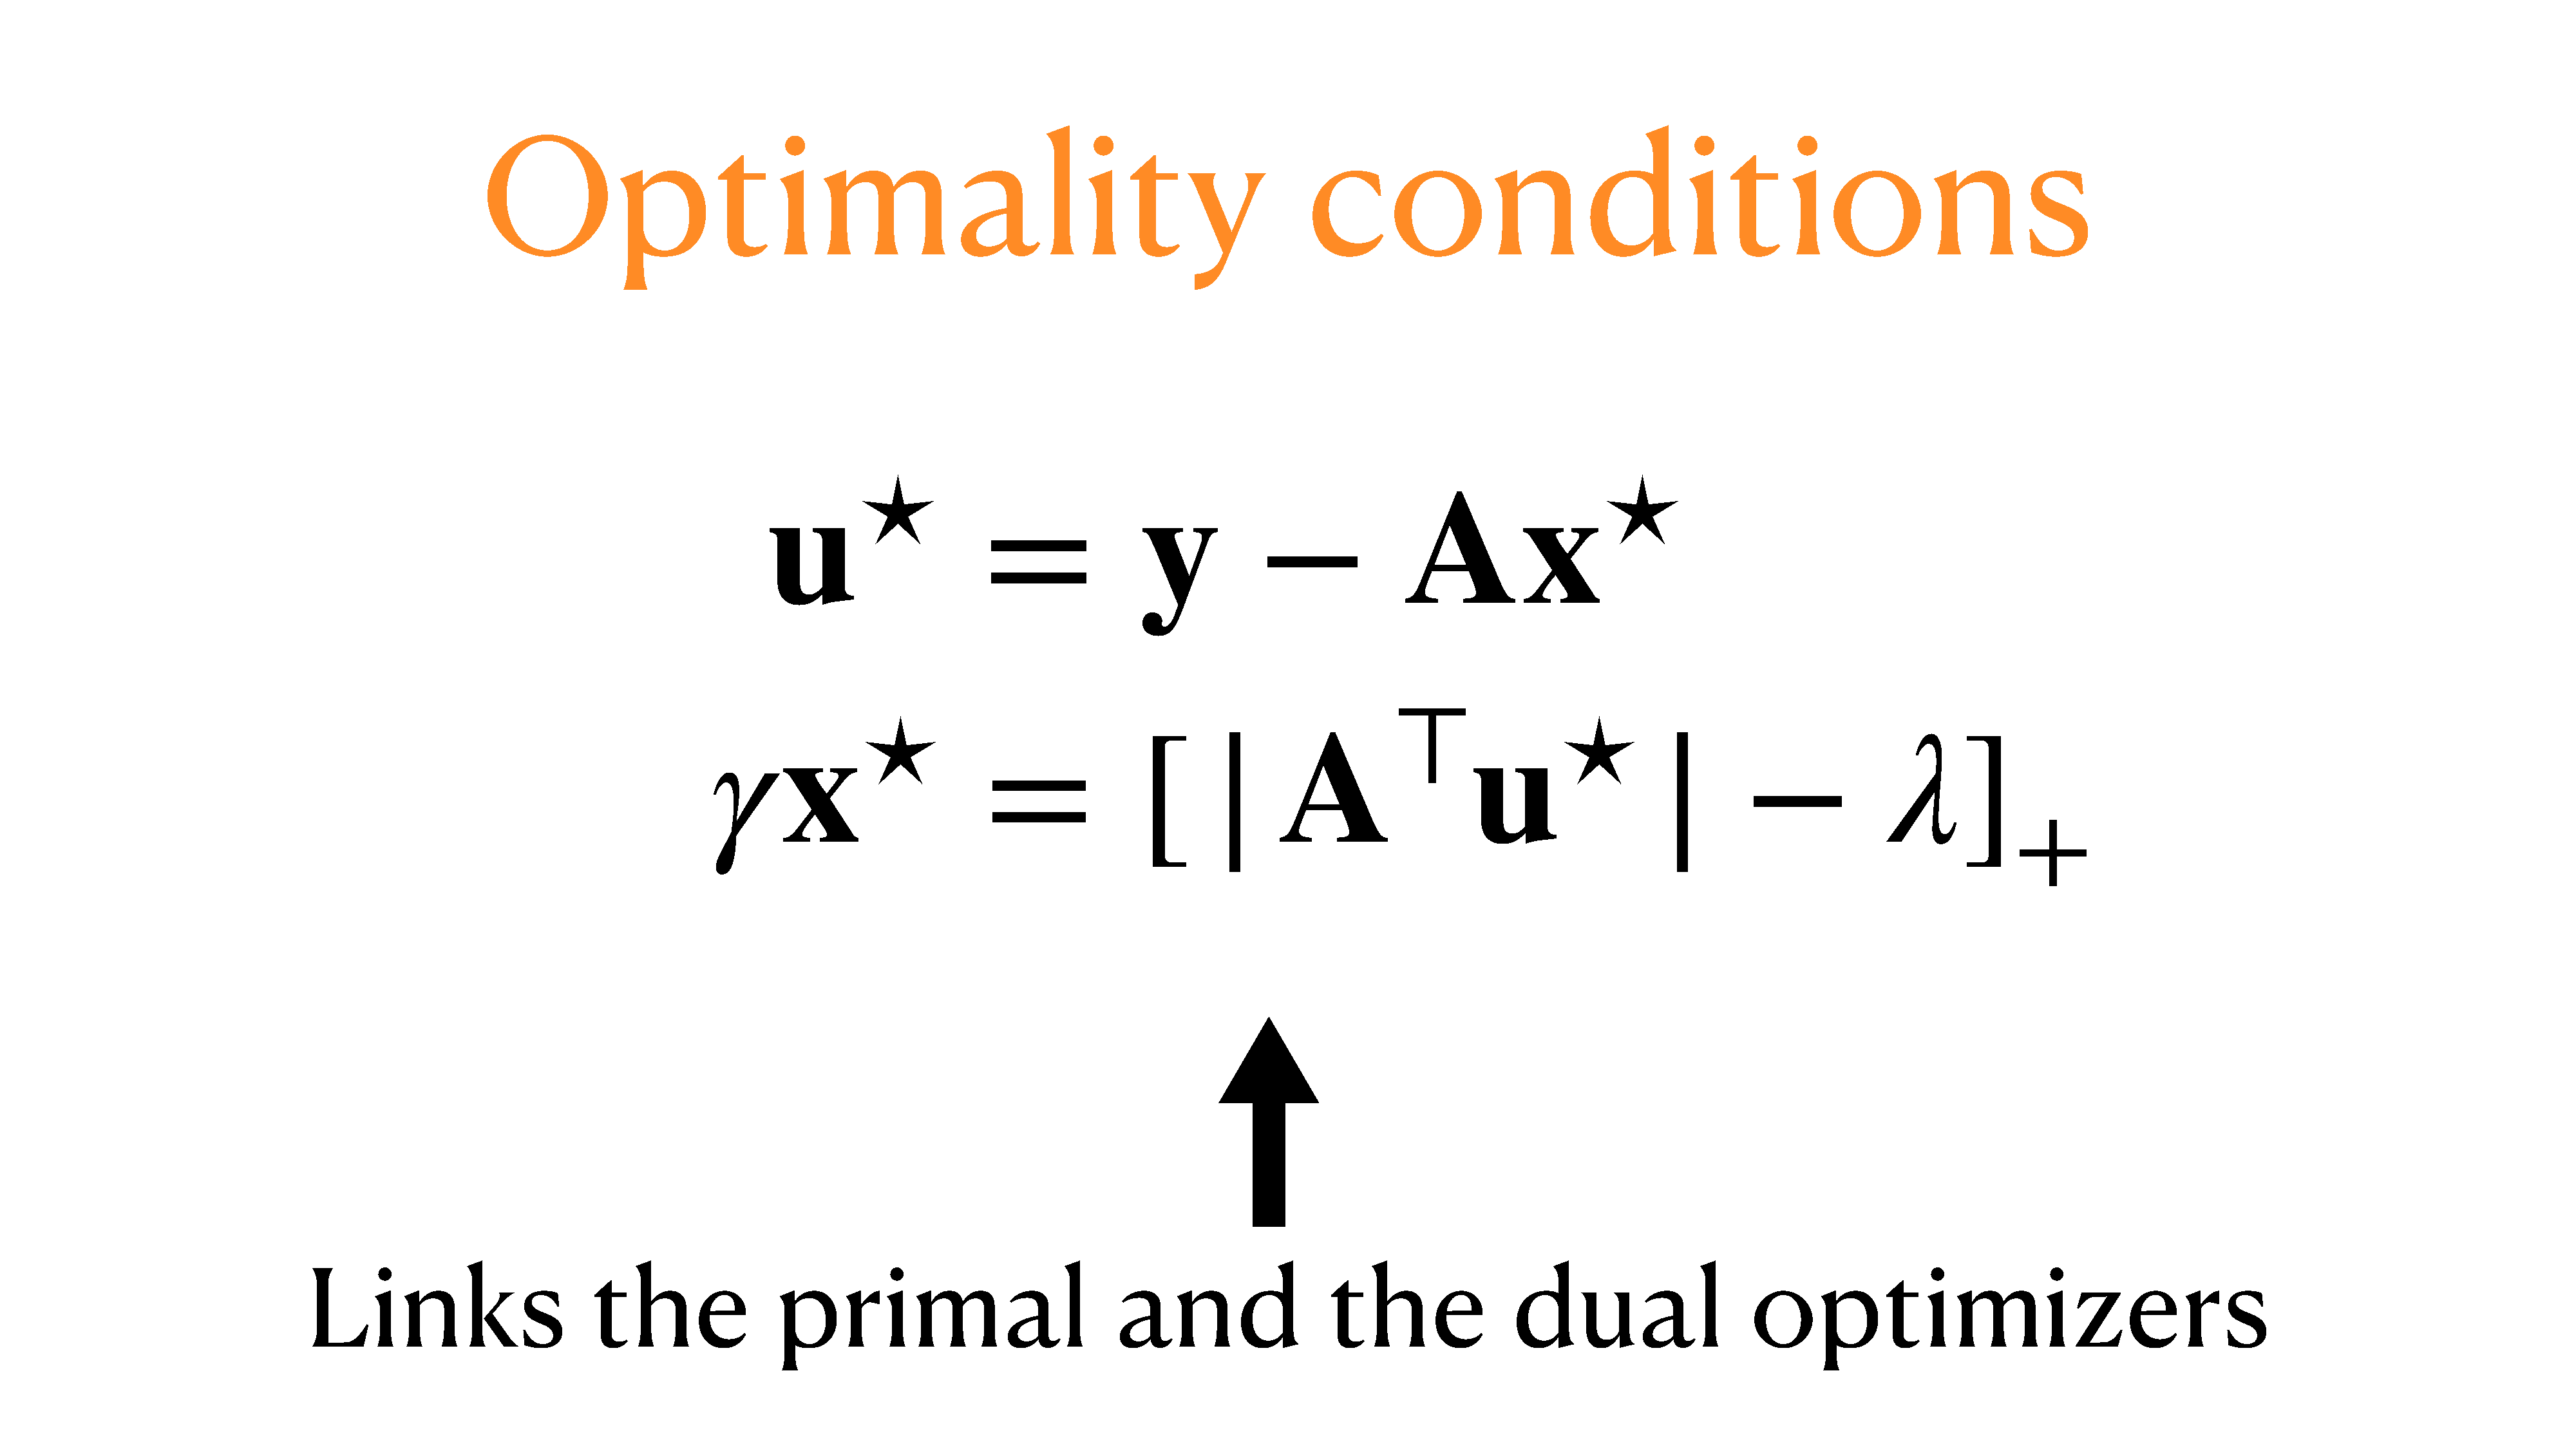
\includegraphics[width=\linewidth]{optcond.pdf}
            \end{column}
        \end{columns}
    \end{block}
    \begin{columns}[t,totalwidth=\twocolwid]
        \begin{column}{\onecolwid}\vspace{-.6in} 
            \begin{alertblock}{Screening tests\\ {\small{(already existing)}}}
                \textbf{Goal :} Identification of \emphone{zeros} in $\pvopt$. \\
                \vspace{0.1in}
                Let $\safesphere(\spherec,\spherer)$ be a sphere containing $\dvopt$, then
                \begin{equation} 
                    \label{eq:screening-test}
                    \forall \idxpvel, \quad |\ktranspose{\atom}_\idxpvel\dv| + \spherer < \rego \implies \pvopt_{\idxpvel}=0
                \end{equation}
                Elements that have passed the screening test can be discarded safely from the problem, as well as the corresponding columns in $\dic$.
            \end{alertblock}
        \end{column}
        \begin{column}{\onecolwid}\vspace{-.6in}
            \begin{alertblock}{Relaxing tests\\ {\small{(our contribution)}}}
                \textbf{Goal :} Identification of \emphone{non-zeros} in $\pvopt$. \\
                Let $\safesphere(\spherec,\spherer)$ be a sphere containing $\dvopt$, then
                \begin{equation} 
                    \label{eq:relaxing-test}
                    \forall \idxpvel, \quad |\ktranspose{\atom}_\idxpvel\dv| - \spherer > \rego \implies \pvopt_{\idxpvel}\neq0
                \end{equation}
                Elements that have passed the relaxing test can be expressed as a linear combination of all the other elements of $\pv$ in the problem.
            \end{alertblock}
        \end{column}
    \end{columns}
    \begin{columns}[t,totalwidth=\twocolwid]
        \begin{column}{\onecolwid}
            \begin{block}{Screen \& Relax strategy}
                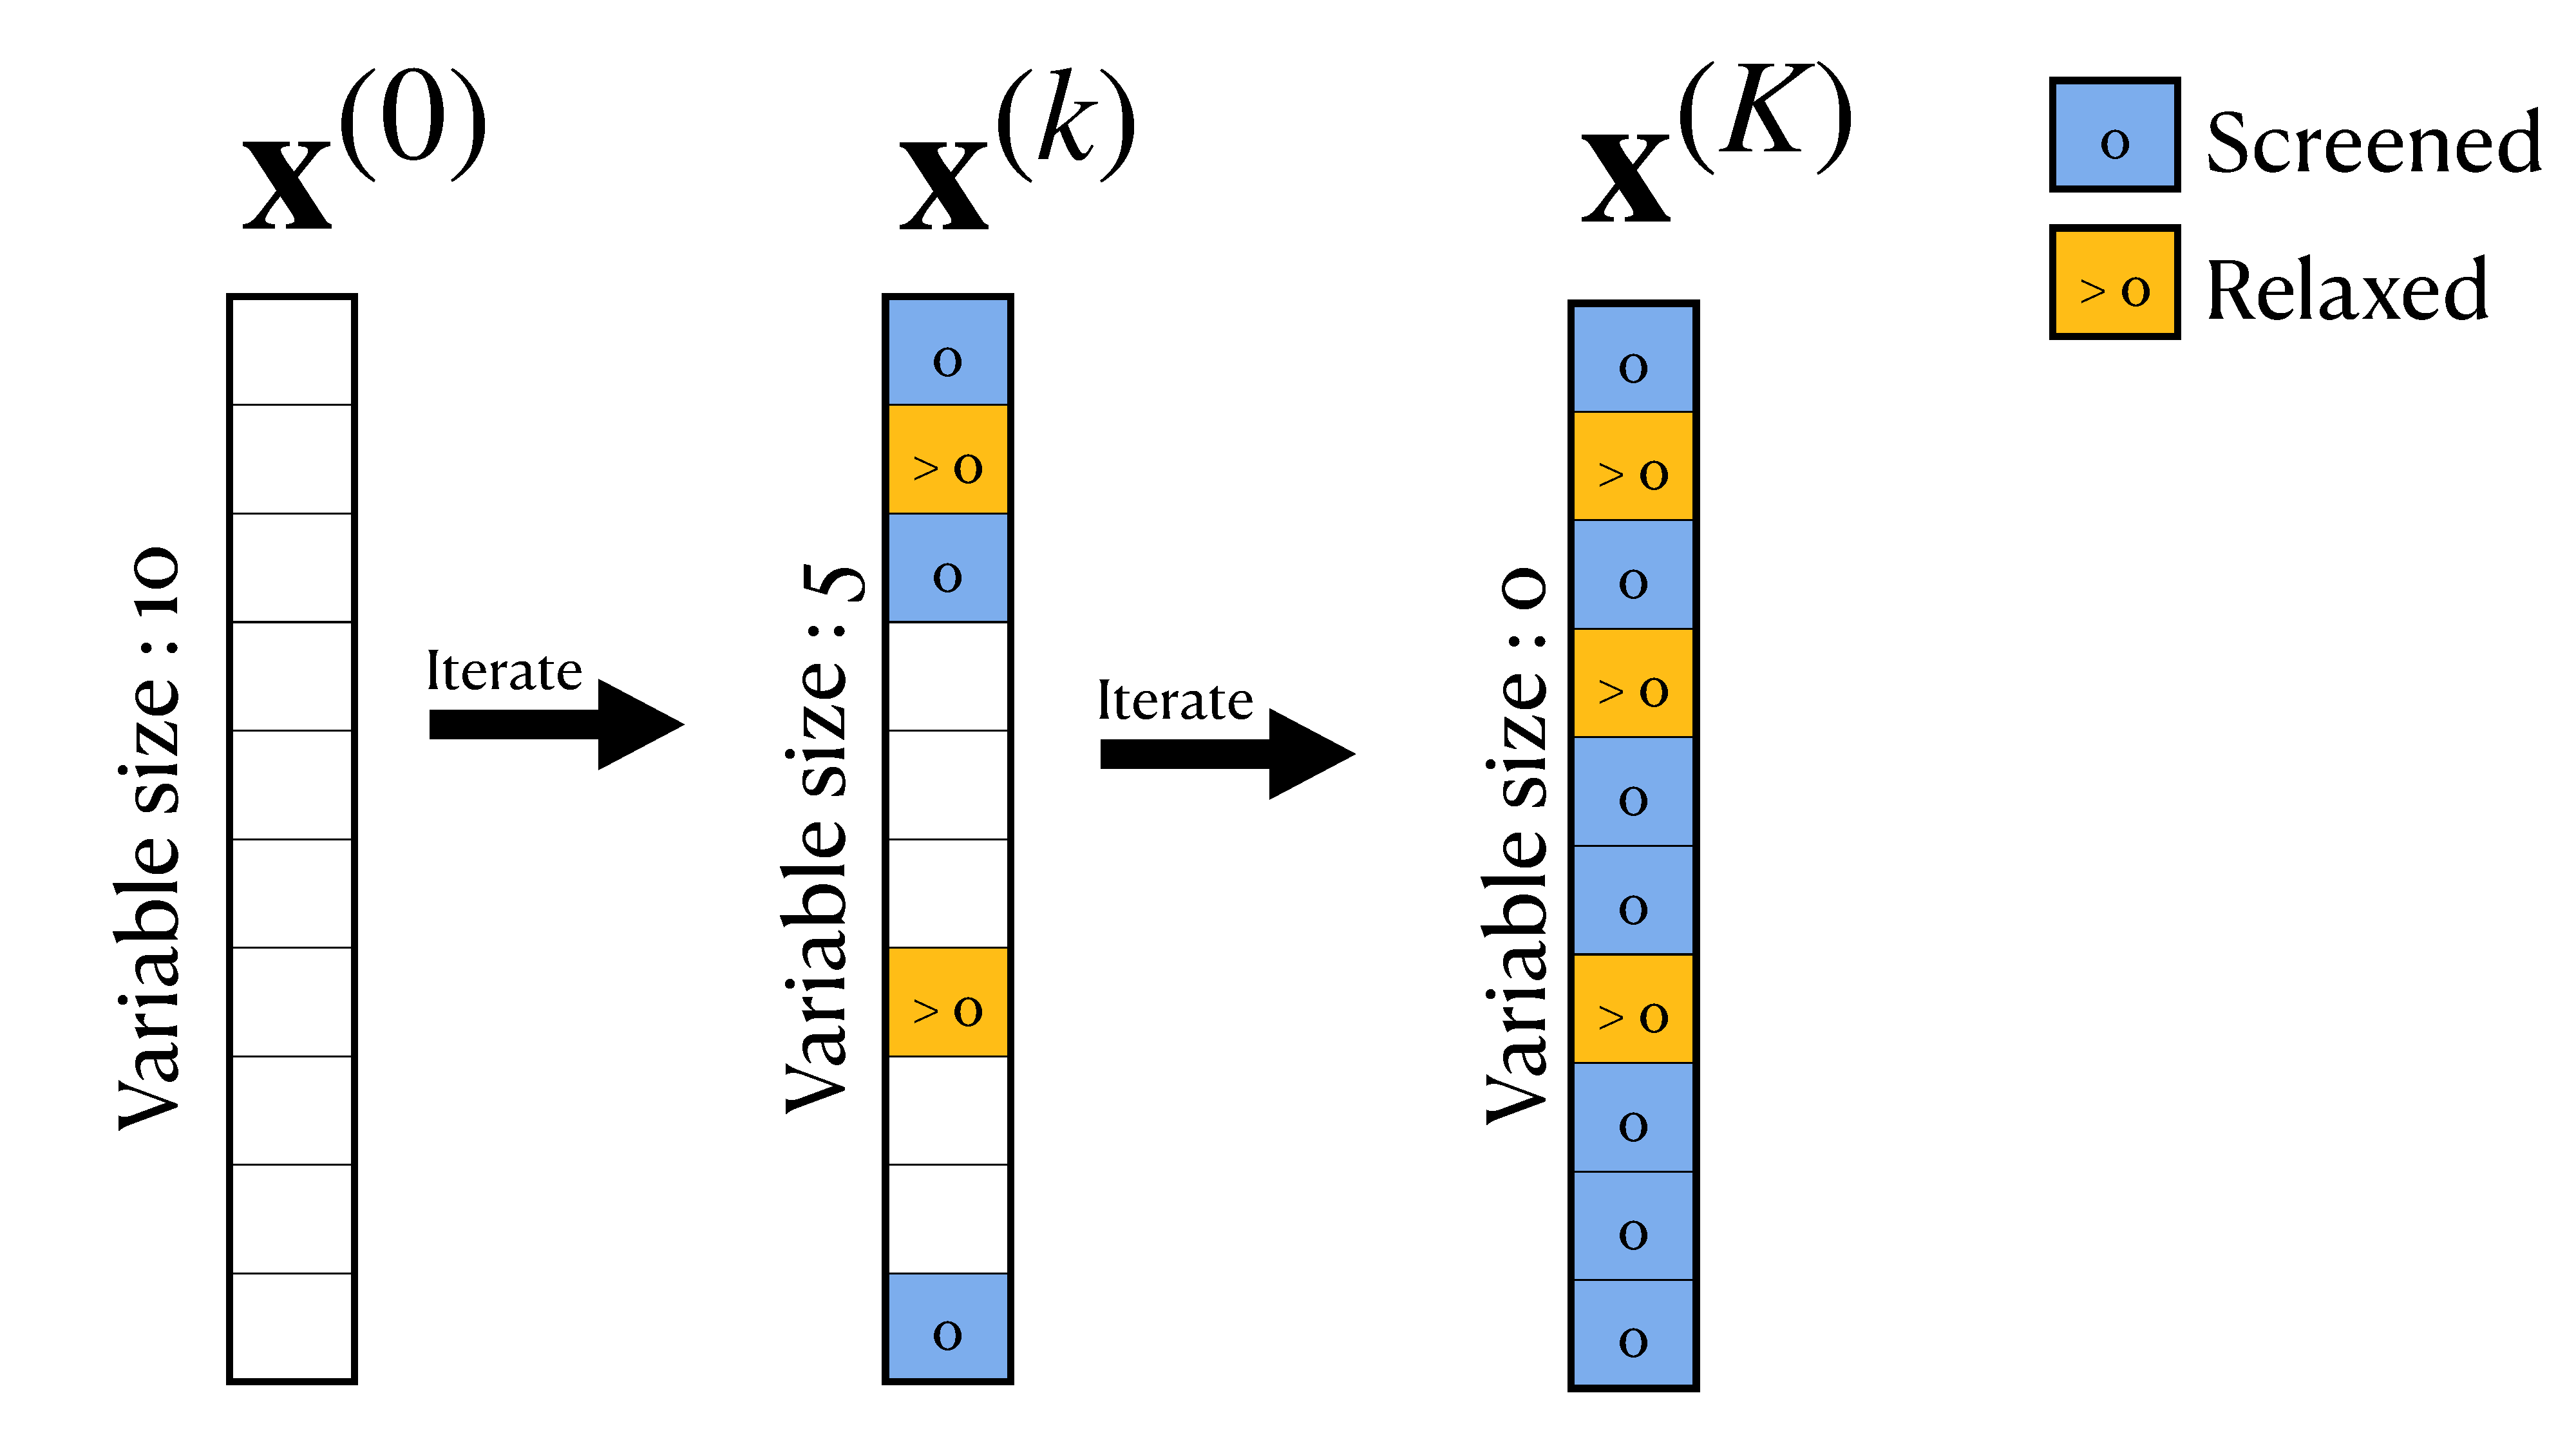
\includegraphics[width=\linewidth]{reduction.pdf}
                \begin{itemize}
                    \item \hspace{0.1in} Benefits of the Screen \& Relax strategy :
                    \begin{itemize}
                        \normalsize \item[-] \hspace{0.1in}\normalsize Dimension shrinking
                        \item[-] \hspace{0in} \normalsize Iteration complexity reduction
                        \item[-] \hspace{0in} \normalsize Conditioning improvement
                        \item[-] \hspace{0in} \normalsize Closed form solution when all elements have been either screened or relaxed
                    \end{itemize}
                \end{itemize}
            \end{block}
        \end{column}
        \begin{column}{\onecolwid}
            \begin{block}{Pseudo-code}
                \begin{algorithm}[H]
                    %\small
                    \DontPrintSemicolon
                    \SetKwInOut{Input}{Input}

                    \BlankLine
                    \Input{Problem data ($\dic,\obs,\rego,\regt$)}
                    \BlankLine

                    \While{convergence is not met}{
                    %
                    Update the current iterate $\pv^{(t)}$ \;
                    Construct a new safe sphere $\safesphere(\spherec^{(t)},\spherer^{(t)})$ \;
                    Perform the screening and relaxing tests\;
                    If new elements have been \emphone{screened}, discard them from the problem\;
                    If new elements have been \emphone{relaxed}, express them as a function of the others. This requires a \emphone{modification of the problem data} that can be done efficiently using \emphone{rank-one rules}.
                    }
                    \caption{Iterative method for the Elastic-Net problem enhanced with a ``Screen \& Relax'' strategy.}
                \end{algorithm}
            \end{block}
        \end{column}
    \end{columns}
\end{column}

\begin{column}{\sepwid}\end{column}

\begin{column}{\onecolwid}

\begin{block}{Numerical results}

    \begin{itemize}
        \item \hspace{0.1in} Data generation :
        \begin{itemize}
            \normalsize \item[1)] \hspace{0.1in} \normalsize Generate a random matrix $\dic \in \kR^{\ddim\times\pdim}$ with either a low or an high correlation between the columns
            \item[2)] \hspace{0.1in} \normalsize Generate a sparse vector $\pv^{\dagger} \in \kR^{\pdim}$
            \item[3)] \hspace{0.1in} \normalsize Set $\obs = \dic\pv^{\dagger} + \text{noise with 10dB SNR}$
            \item[4)] \hspace{0.1in} \normalsize Calibrate $\lambda$ and $\gamma$ statistically
        \end{itemize}
    \end{itemize}
    ~\\
    \begin{itemize}
        \item \hspace{0.1in} Concurrent methods :
        \begin{itemize}
            \normalsize \item[-] \hspace{0.1in} \normalsize Proximal-Gradient (PG) algorithm
            \item[-] \hspace{0.1in} \normalsize PG algorithm with \emphone{screening}
            \item[-] \hspace{0.1in} \normalsize PG algorithm with \emphone{relaxing}
            \item[-] \hspace{0.1in} \normalsize PG algorithm with \emphone{screening and relaxing}
        \end{itemize}
    \end{itemize}
    ~\\
    \hspace*{-2em}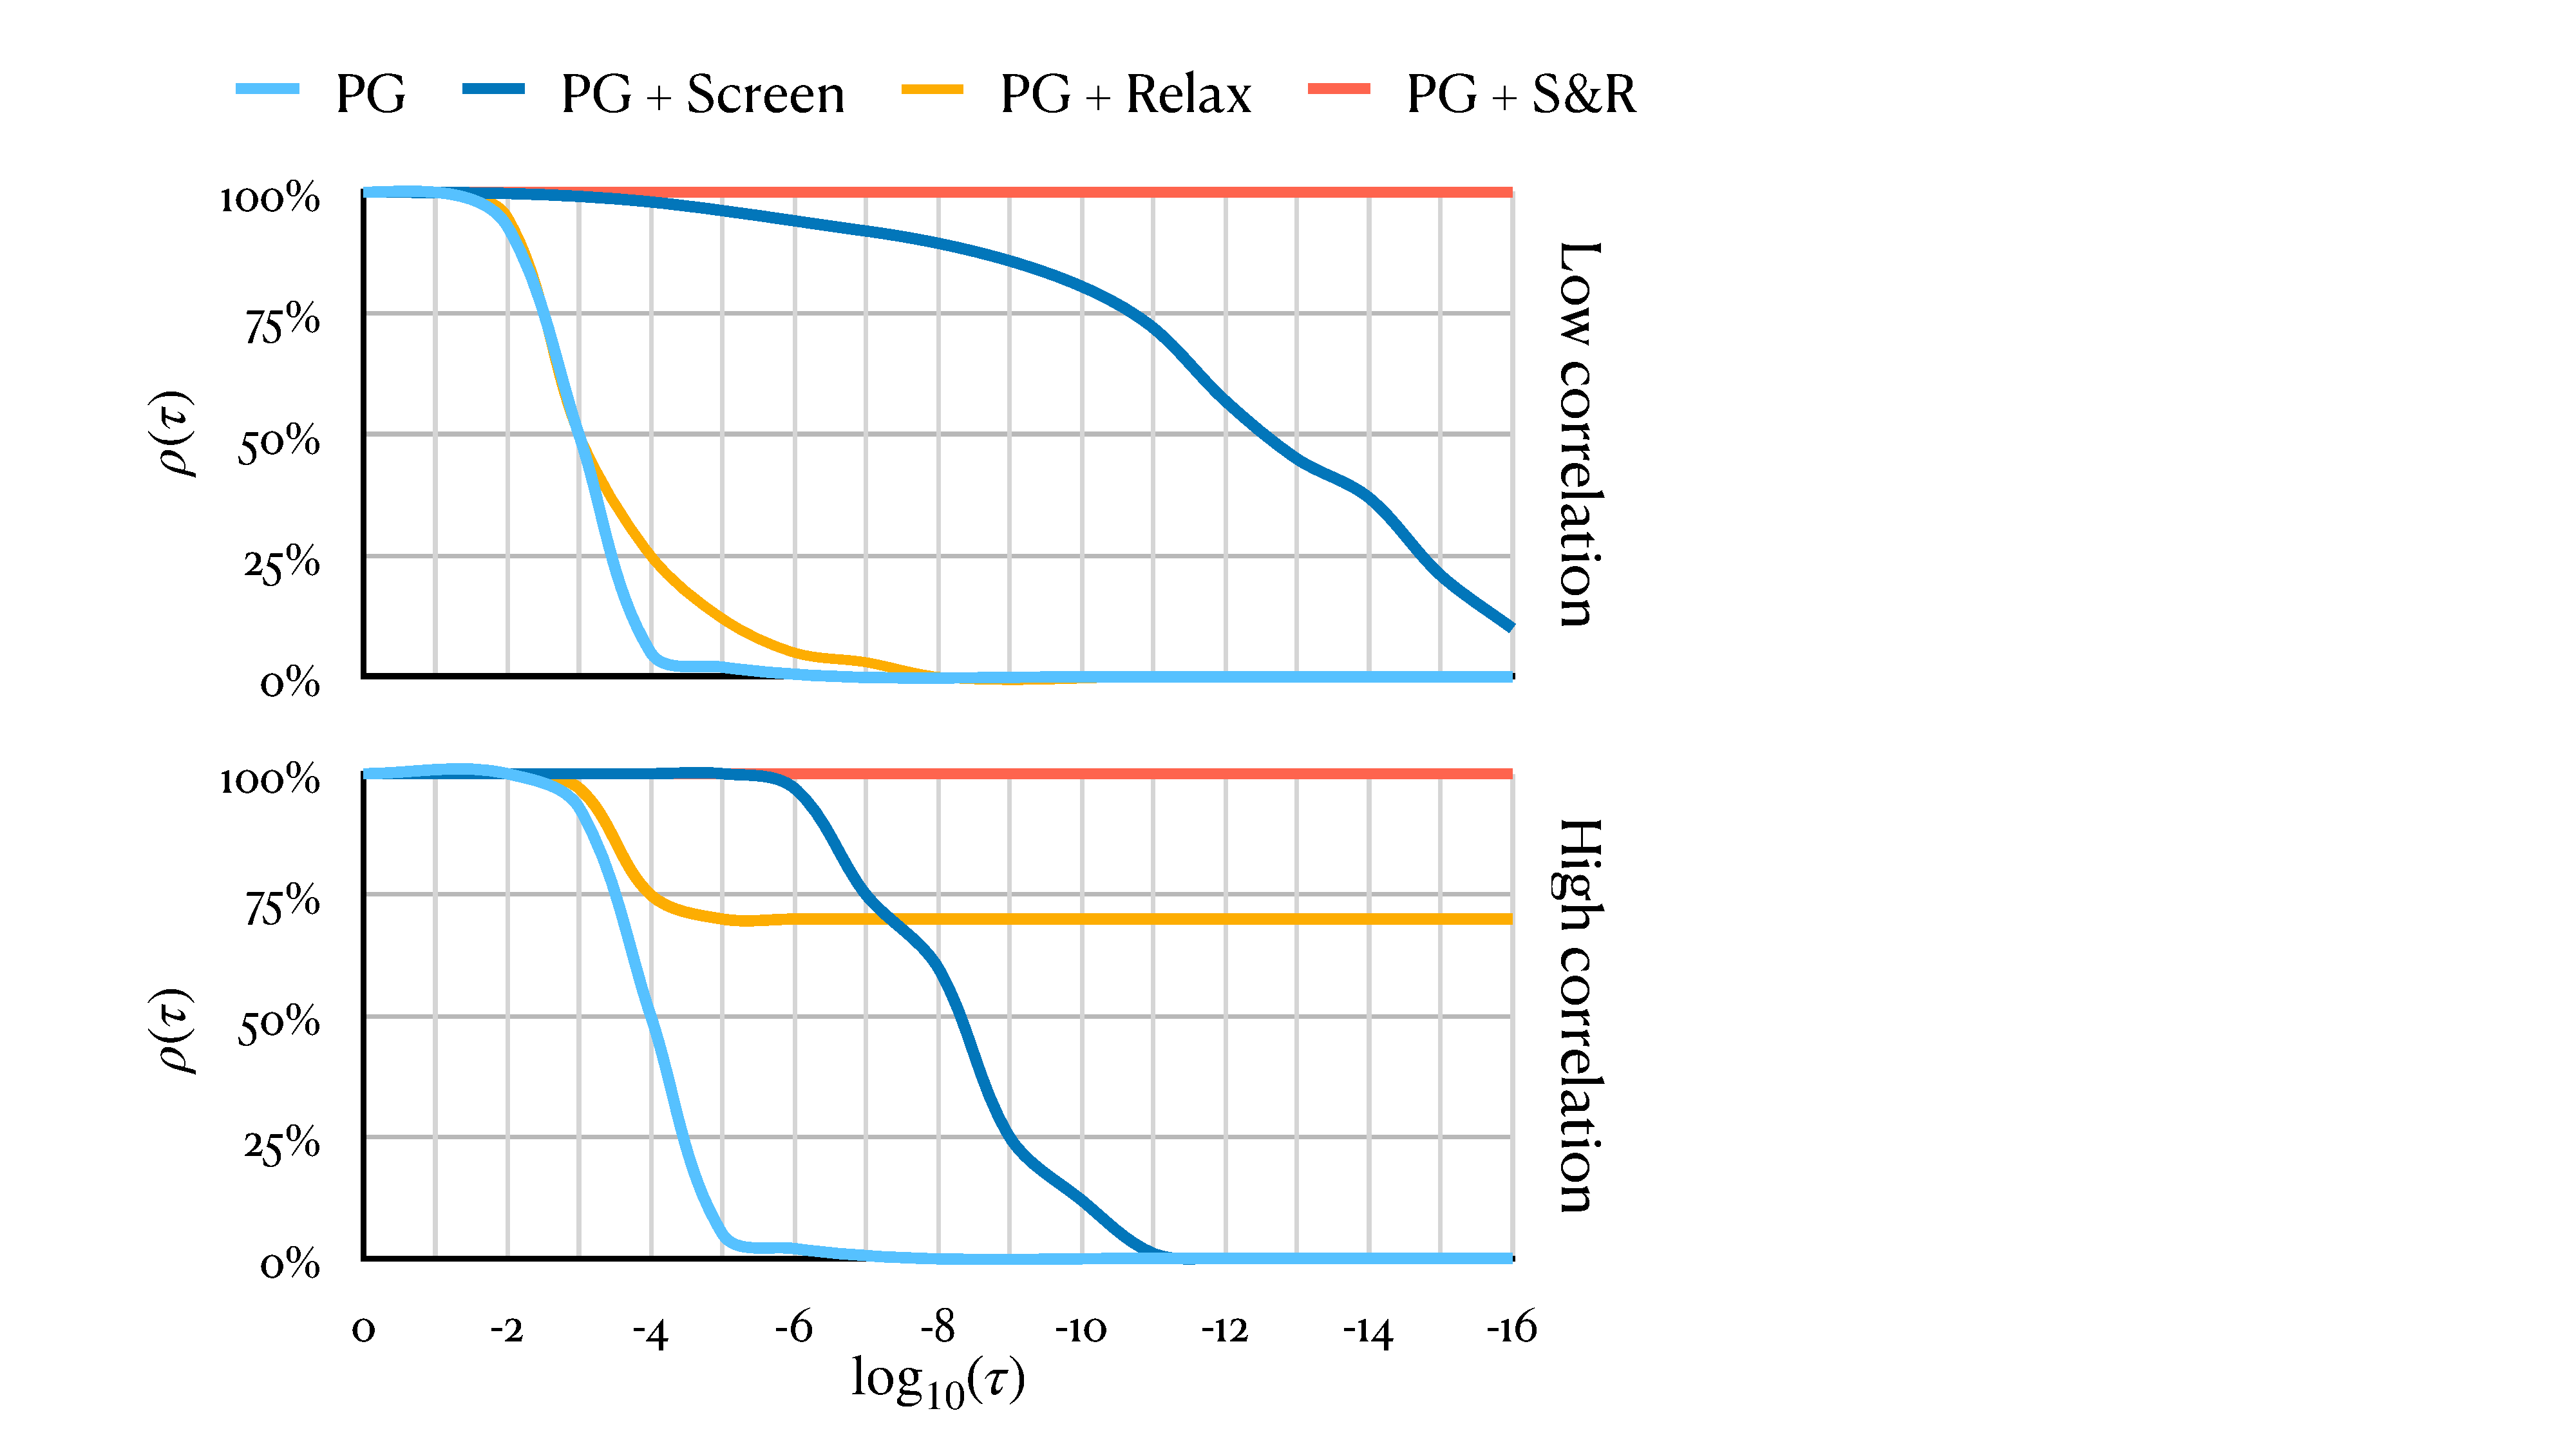
\includegraphics[width=1.7\linewidth]{plot.pdf}
    
    \begin{itemize}
        \item \hspace{0.1in} Observations :
        \begin{itemize}
            \normalsize \item[-] \hspace{0.1in} \normalsize Screening only : efficient when correlation between the columns is \emphone{low}.
            \item[-] \hspace{0.1in} \normalsize Relaxing only : efficient when correlation between the columns is \emphone{high}.
            \item[-] \hspace{0.1in} \normalsize Screening and Relaxing : allows convergence up to machine precision in all the setups tested.
        \end{itemize}
    \end{itemize}
    \vspace{1em}
    \textbf{Take home message :} Both the identification of \emphone{zero} and \emphone{non-zero} elements in the Elastic-Net solution allows to enhance its resolution.

\end{block}

\end{column} 

\begin{column}{\sepwid}\end{column}

\end{columns}
\end{frame}
\end{document}
